\newcommand{\mysection}[1]{\vspace{-.00cm}\section{#1}\vspace{-.00cm}}
\newcommand{\mysubsection}[1]{\vspace{-.00cm}\subsection{#1}\vspace{-.00cm}}
\newcommand{\mysubsubsection}[1]{\vspace{-.00cm}\subsubsection{#1}\vspace{-.00cm}}

%\documentclass{acm_proc_article-sp}
\documentclass[12pt]{article}

\usepackage{multirow}
\usepackage{times}
\usepackage[scaled=0.92]{helvet}
\usepackage[T1]{fontenc}
\usepackage{enumerate}
\usepackage{textcomp}
\usepackage{graphicx}
\usepackage[pdftex]{hyperref}
\usepackage{url}
\usepackage{mathptmx}
\usepackage{bbm}
\usepackage{dsfont}
\usepackage{subfig}
\usepackage[noadjust]{cite}
\usepackage{amsmath}
\usepackage{array}
\usepackage{fancyvrb}
\usepackage{listings}
\usepackage{xcolor}
\usepackage{caption}
\usepackage[super]{nth}

\DeclareCaptionFont{white}{\color{white}}
\DeclareCaptionFormat{listing}{%
  \parbox{\textwidth}{\colorbox{gray}{\parbox{\textwidth}{#1#2#3}}\vskip-4pt}}
\captionsetup[lstlisting]{format=listing,labelfont=white,textfont=white}
\lstset{frame=lrb,xleftmargin=\fboxsep,xrightmargin=-\fboxsep}

\begin{document}
\title{Assignment 2 Solutions}
\date{\today}

%\numberofauthors{1}
%\author{
%\alignauthor Aaron Cahn\\
%\affaddr{University of Wisconsin-Madison}\\
%\email{cahn@cs.wisc.edu}
%}


\author{
Aaron Cahn\\
University of Wisconsin-Madison\\
cahn@cs.wisc.edu
}

\maketitle

\newpage
\section{Solutions} \label{sec:solutions} \subsection{Question 1}
\subsubsection{Part A}

Let \(A\) be a symmetric matrix of dimension \(m\).
The entries of \(A\) are denoted by \(a_{ij}\).

\begin{eqnarray}
  A = 
  \begin{bmatrix}
    a_{11} & \dots & a_{1j} \\
    \vdots & & \vdots \\
    a_{i1} & \dots & a_{ij} \\
  \end{bmatrix}
  \label{eqn:syma}
\end{eqnarray}

After one iteration the first row of \(A\) will be unchanged and the first column will contain zeros below the first element.
The \((m-1)x(m-1)\) sub matrix of \(A\) is computed by the equation \(a_{ij} = a_{ij} - \frac{a_{i1}}{a_{11}}*a_{1j}\).
Since, \(A\) is a symmetric matrix \(a_{ij} = a_{ji}\).
Therefore this submatrix will remain symmetric because the equation to compute \(a_{ji}\) is the same as the equation to compute \(a_{ij}\) listed above.
The next iteration of \(LU\) factorization is now operating on this symmetric matrix so we can simply relable the elements of the submatrix is we did in \ref{eqn:syma} because we can ignore the first row and first column of \(A\).

Therefore, the same argument applies for the second iteration.
By induction it can then be shown that after iteration \(k\) the \((m-k)x(m-k)\) sub matrix of the \((m-k+1)x(m-k+1\) sub matrix of \(A\) is symmetric.
Explicitly the computation of the sub matrix is \(a_{ij} = a_{ij} - \frac{a_{ik}}{a_{kk}}*a_{kj}\).
From this it is clear the \((m-k)x(m-k)\) sub matrix is still symmetric because we have proven above the \((m-k+1)x(m-k+1)\) sub matrix of \(A\) after iteration \(k-1\) is symmetric ({\em e.g.,} if we unroll to where \(k=1\)).
This concludes the proof.

\newpage
\subsubsection{Part B}

\lstinputlisting[caption=Matlab Commands,showstringspaces=false,language=Matlab]{../lu_sym.m}

\subsubsection{Part C}
The complexity of Gauss elimination is is \(O(\frac{m^{3}}{3})\).
Regular gauss elimination works on an entire matrix ({\em i.e.,} touching all elements of the matrix) during \(LU\) factorization.
However, for a symmetric matrix we have proven in part A that we only need to touch the upper triangular elements of a matrix.
This constitutes half of the matrix.
Therefore, the complexity of the symmetric \(LU\) factorization algorithm will be \(\frac{1}{2}\frac{m^{3}}{3}\) or simply \(O(\frac{m^{3}}{6})\).

\newpage
\subsubsection{Part D}

\lstinputlisting[caption=Matlab Commands,showstringspaces=false,language=Matlab]{../q1_partD.m}
\lstinputlisting[caption=Matlab Commands,showstringspaces=false,language=Matlab]{../q1_partD_results}

It is clear from the results that the ratio between the run time of the symmetric \(LU\) factorization script over the Gauss elimination \(LU\) factorization script is converging to \(\frac{1}{2}\).
This confirms the complexity predicted for symmetric \(LU\) factorization in part C of this question.
Note, experiments were run on symmetric matrices with \(m \in \{30,40,50,60 \}\).

\newpage
\subsection{Question 2}

\subsubsection{Part A}
This code does the basic Gauss elimination \(LU\) factorization.
It is the same code used in question 1 during the comparison to the symmetric \(LU\) factorization.

\lstinputlisting[caption=Matlab Commands,showstringspaces=false,language=Matlab]{../lu_basic.m}

\subsubsection{Part B}
As stated in the question, we simply use Matlab's lu routine to accomplish this algorithm.
Note, Matlab's lu routine does partial pivoting.

\newpage
\subsubsection{Part C}

This code does complete pivoting before Gauss elimination.
The code returns [L,U,P,Q] where \(P\) and \(Q\) are permutation matrices.
The algorithm produces matrices for the equation \(PAQ = LU\). 

\lstinputlisting[caption=Matlab Commands,showstringspaces=false,language=Matlab]{../lu_pivot.m}

\newpage
\subsubsection{Part D}

The code below is the experimental setup that was run to obtain results for this question.

\lstinputlisting[caption=Matlab Commands,showstringspaces=false,language=Matlab]{../q2_partD.m}

The code below is the output from the experimental setup above and represents the results from the experiment.

\lstinputlisting[caption=Matlab Commands,showstringspaces=false,language=Matlab]{../q2_partD_results}

From the experimental analysis we can see that the first two matrices are very poorly conditioned.
Therefore, there is no hope of obtaining a correct answer even before \(LU\) factorization is performed in any fasion.
This is to say the conditioning of the original matrix \(A\) is so bad there the stability of the algorithms does not matter.

The next issue is that of stability.
It is clear from the experiments that the stability of the algorithms improves in the order Gauss Elimination, partial pivoting, and then full pivoting being the most stable.
Note, the complexity increases in the same manner ({\em i.e.,} full pivoting is the most costly algorithm).
This is evident from the errors dropping from one algorithm to the next.
The stability does not improve drastically between partial and full pivoting.
Note, this is only really relevant for matrices that are not poorly conditioned.

The final issue is that of conditioning and stability on random matrices.
It is almost always the case that the conditioning of a random matrix \(A\) will be good.
This is because the probility of randomly creating to vectors that are linearly dependent is so low, and this increases as the size of the matrix increases.
Therefore, the penalty incurred by using a more stable algorithm is generally not worth it for a random matrix.

\newpage
\subsection{Question 3}
\subsubsection{Part A}

\lstinputlisting[caption=Matlab Commands,showstringspaces=false,language=Matlab]{../q3_partA}

As we see above, after we deflate \(v\) from \(A\) we obtain,
\begin{eqnarray}
  A_1 = 
  \begin{bmatrix}
    7 & 0 & 0 \\
    0 & 9 & -6 \\
    0 & 6 & -6 \\
    \end{bmatrix}
\end{eqnarray}

\newpage
\subsubsection{Part B}

\lstinputlisting[caption=Matlab Commands,showstringspaces=false,language=Matlab]{../q3_partB}

As we see above the eigen pairs of \(\tilde{A}_1\) are,

\begin{eqnarray}
  e_1 = \left(6,
  \begin{bmatrix}
    0.8944 \\
    0.4472 \\
  \end{bmatrix}
  \right),
  e_2 = \left(-3,
    \begin{bmatrix}
      0.4472 \\
      0.8944 \\
    \end{bmatrix}
  \right)
\end{eqnarray}

\newpage
\subsubsection{Part C}

\lstinputlisting[caption=Matlab Commands,showstringspaces=false,language=Matlab]{../q3_partC}

Therefore, \(v_1, v_2, v_3\) are the eigenvectors of \(A\).
They are all normalized and therefore form an eigenbasis of \(A\) to \(\mathbb{R}^{3}\).
The eigenbasis is thus,

\begin{eqnarray}
  \left(
    \begin{bmatrix}
    0.8571 \\
    0.4286 \\
    0.2857 \\
    \end{bmatrix}
    ,
    \begin{bmatrix}
      0.5111 \\
      -0.6389 \\
      -0.5750 \\
    \end{bmatrix}
    ,
    \begin{bmatrix}
      0.4472 \\
      -0.8944 \\
      0 \\
    \end{bmatrix}
    \right)
\end{eqnarray}

\newpage
\subsubsection{Part D}

We can simply use the eigenbasis from above to form the matrix \(P\).
The matrix \(D\) is simply the eigenvalues \(l_1,l_2,l_3\) from above.
Therefore we have diagonalized \(A\).
Note, we use Matlab to compute \(P^{-1}\).

\begin{eqnarray}
  P = 
  \begin{bmatrix}
    0.8571 & 0.5111 & 0.4472 \\
    0.4286 & -0.6389 & -0.8944 \\
    0.2857 & -0.5750 & 0 \\
  \end{bmatrix}
  ,
  D = 
  \begin{bmatrix}
  7 & 0 & 0 \\
  0 & 6 & 0 \\
  0 & 0 & -3 \\
  \end{bmatrix}
  ,
  P^{-1} = 
  \begin{bmatrix}
    0.8571 &  0.4286 &  0.2857 \\
    0.4259 &  0.2130 & -1.5972 \\
    0.1065 & -1.0648 &  1.2778 \\   
  \end{bmatrix}
\end{eqnarray}

\lstinputlisting[caption=Matlab Commands,showstringspaces=false,language=Matlab]{../q3_partD}


%\begin{figure}[th]
%  \centering
%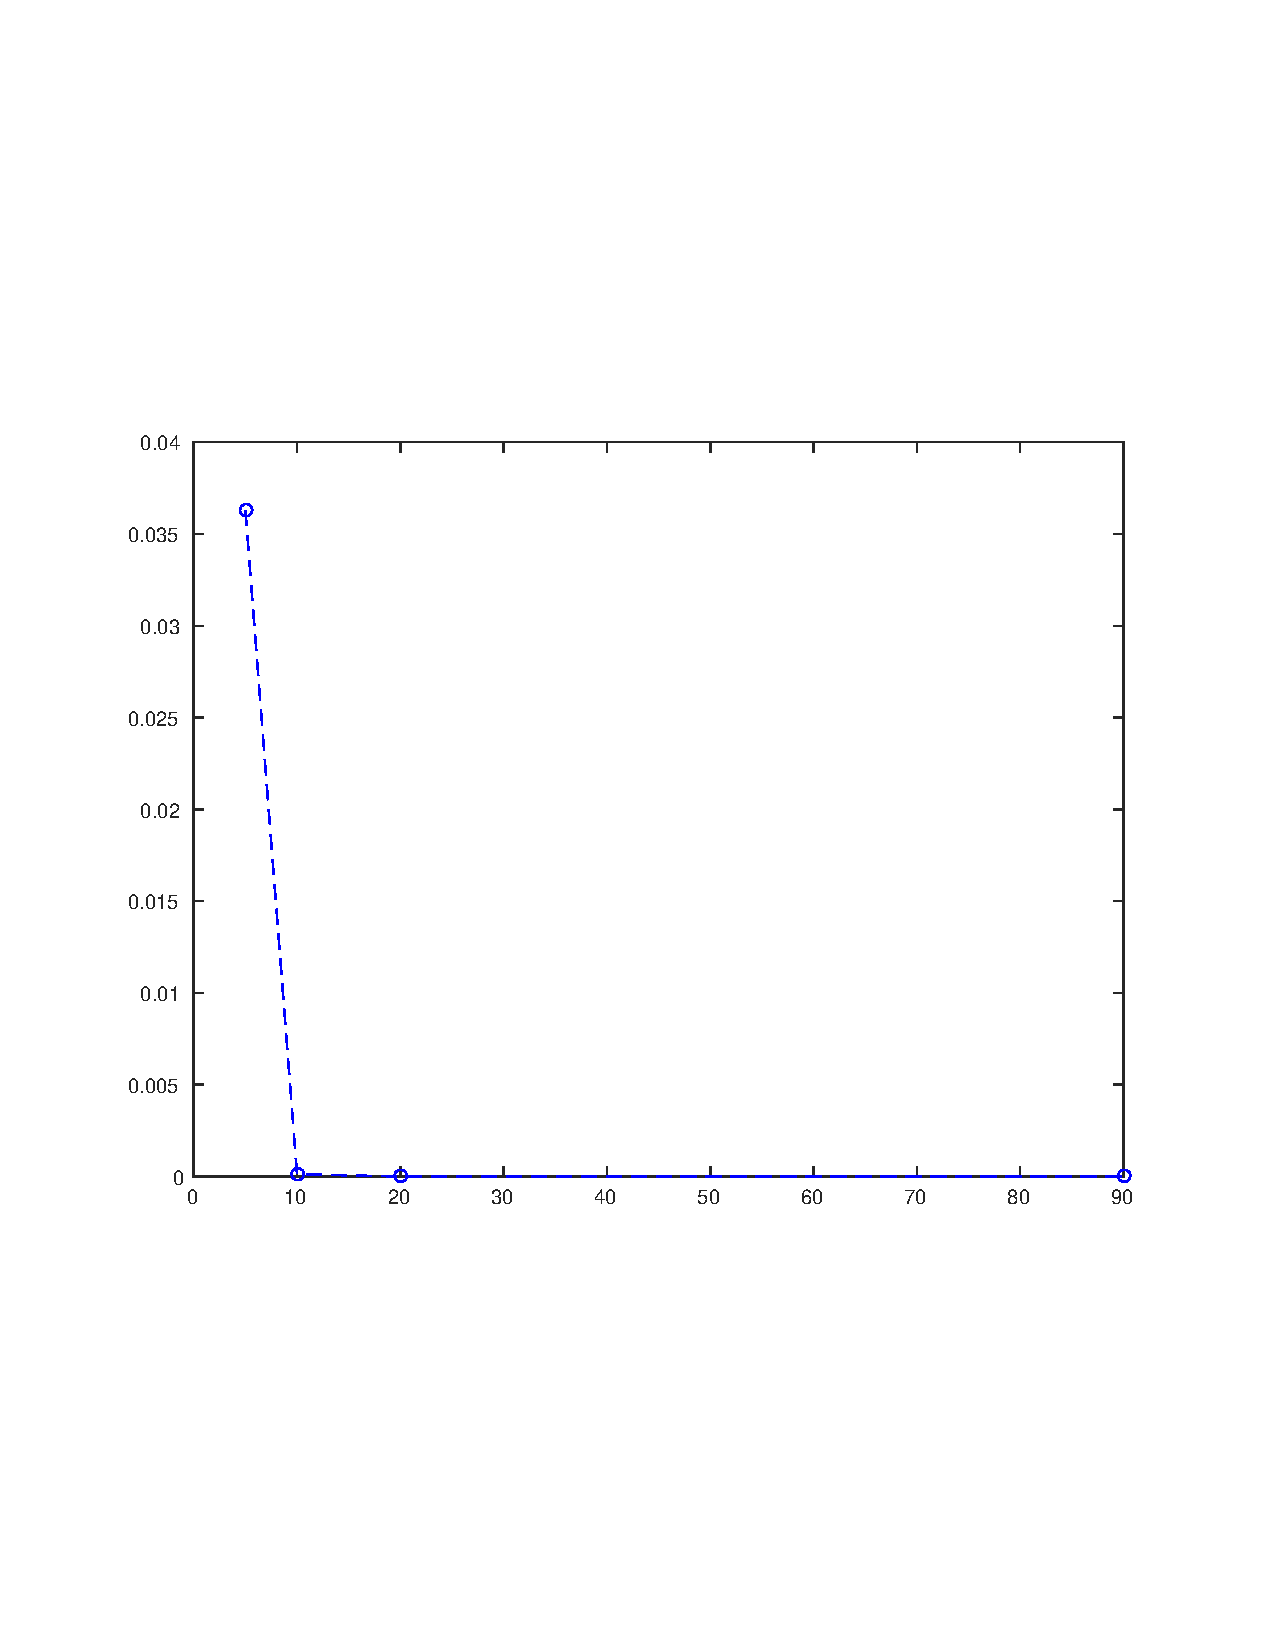
\includegraphics[trim=10mm 70mm 10mm 70mm, width=1.0\textwidth]{../q2_plots}
%\end{figure}


%\bibliographystyle{plain}
%\bibliography{paper}

\end{document}
